\section{Sprint 4}

This is the last sprint. We have all the main features of the game implemented, this phase will focus on the feedback from the customer and the usability test and to implement a few features that adds flavor to the game, like sound and high score.

\subsection{Sprint Planning}

	This is the last sprint where new features will be implemented. We plan to implement the last 
	requirements which are all rated medium and low. Several necessary improvements and some new 
	features were discovered during the usability test held in sprint 3, and these will be implemented 
	in this sprint. Some time will also be spent fixing bugs.

\subsection{Duration and Workload}

	The goal of this sprint was to finish the game. When finishing the game we focused on closing all
	requirements in the product backlog and do the last part of redesign and bug fixing. The total
	workload is listed here:

	{\bf Duration:} 28.10 - 10.11 (2 weeks)\\
	{\bf Workload:} This is the list with hours spent (the whole group) on the project in this sprint.
	\begin{itemize}
		\item {\bf Planning:}  12 hours
		\item {\bf Development:}  80,5 hours
		\item {\bf Documentation (report):} 52.5 hours
		\item {\bf Testing:} 16 hours
	\end{itemize}
	{\bf Total workload: }  161 hours \\

	In this sprint we managed a workload of 20.1 hours in average per person each week (161 hours/4 persons/2 weeks). We always strive to reach a workload of 20-24 hours and the group managed this 
	at sprint 4.  

\clearpage
\subsection{Sprint Backlog}

	Table \ref{table:backlog4} shows the backlog for sprint 4.

	\begin{table} [H]
	\begin{tabular}{| p{1cm} | p{7cm} | p{2cm} | p{2cm} |}
		\hline
		\rowcolor{gray}
		ID & Description & Estimate & Actual effort \\ \hline
		FR1.2 &  The user should be able to exit the game at any time, and the game state should be saved and loaded when the user returns to the game. 
		& 10 hours & Not implemented. \\ \hline

		FR1.4 & The user should get a high score based on the time spent finishing the level. 
		& 5 hours & 3 hours \\ \hline

		FR1.5 & The user should be able to improve the high score on any level by beating previous high scores. 
		& 2 hours & 2 hours  \\ \hline

		FR1.6 & The user should be able to pause the game at any time. 
		& 7 hours & 5 hours \\ \hline

		FR1.7 & The game should play background music. 
		& 8 hours & 10 hours \\ \hline

		FR1.8 & The user should be able to turn on/off the background music. 
		& 3 hours & 1 hour \\ \hline

		FR1.9 & There should be played a sound effect when the player collects money. 
		& 3 hours & 1.5 hours \\ \hline

		FR1.10 & There should be played a sound effect when the player upgrades the powerplant. 
		& 3 hours & 2 hours \\ \hline

		FR1.11 & There should be played a sound effect when the player builds a power line 
		& 3 hours & 1.5 hours \\ \hline

		FR1.13 & There should be a sound notification for when new obstacles appear. 
		& 3 hours & Not implemented. \\ \hline

		FR1.14 & There should be played a sound effect when the player builds a power plant. 
		& 3 hours & 1.5 hours \\ \hline

		FR2.7 & The player should only be allowed to build a level-specific number of power plants. 
		& 5 hours & Not implemented.  \\ \hline

		FR2.9 & The houses should not appear on top of each other. 
		& 7 hours & 5 hours \\ \hline
		
		FR6.6 & A power preservation tip should appear when the user reaches a new level. 
		& 5 hours & Not implemented. \\ \hline

	\end{tabular}
	\caption{Sprint backlog sprint 4}
	\label{table:backlog4}
	\end{table}

	In this sprint we added all requirements from the product backlog. Because of time constraints,
	and because this is the final sprint of the project, not all of the of these requirements were
	implemented.

	The requirement FR1.2 was not implemented because it had a high cost in terms of implementation
	time, and the group decided the value for the customer was too low to justify the time it would
	take to implement. However, the requirement is partly implemented in the pause functionality.
	The game state is saved when the user exits the game, but the state will be lost when the player
	turns off the phone. This will be added to ``further work''.

	When the group designed the game, we wanted to add a notification when a new obstacle appeared
	outside the gamescreen (FR1.13). We wanted to have a pointer on the screen so the player knew
	where the new notification appeared. This is only partly implemented in terms of sound. There
	is a sound effect when a new obstacle appears, but the player will not get the direction.

	The group added a requirement that should limit the number of power plants it's possible to
	build during a level (FR2.7). The group decided that this was not necessary because if the
	player builds too many power plants, the player will not get to the next level. Because of this,
	we did not implement this requirement.

	The project description which was handed out at the start of this project stated that power
	preservation tips should be included in the game (FR6.6). During the first customer meeting,
	the customer told the group that this was not very important, and that this requirement was
	suggested by course staff and not something that they themselves had required. We will add
	this to ``further work'', and we have made some space on the ``victory screen'' where this can
	be added if Helgelandskraft should change their mind. In terms of working hours, this is a
	fairly easy implementation.

\subsection{Implementation}

	\subsubsection*{jQuery UI}

	We used jQuery UI to implement pop-up and dialog messages when we need to give text feedback to the player or ask the player to choose between options during gameplay. jQuery UI can be customized and gives us more flexibility than the JavaScript native window alerts. Also, the jQuery UI dialog messages does not block computation while waiting for user input\cite{jqueryui}.

	\subsubsection*{Pause game}

	The game is properly paused when the player presses the "home" button, or a
	similar button which puts the game in the background. There is also a
	dedicated button to pausing the game that the player can press while
	playing, allowing the player to leave the game at any time without
	consequences.

	\subsubsection*{Audio}

	Sound effects are played when the player build power plants, upgrade
	power plants, build power lines or collect money.When collecting money a
	random sound from a list of sounds is played.

	\subsubsection*{High score}

	When the user successfully finishes a level, they get a score depending on
	how much time they spent on the level. If the player spent less time on that
	level than they did previously, then the new score is added to the high score
	list.

	\subsubsection*{Building placement}

	Originally buildings was placed randomly around the map. They could appear
	on top of each other. This created problems for the player when attempting
	to connect the buildings with power lines or collecting money. To avoid
	this, we created a list of possible building locations and shuffled it. Then
	when the game places new buildings it takes them from this list. The player
	is also incapable of building power plants on top of already existing
	buildings.
	
\begin{figure}[H]
	\centering
	\subfigure{
		
\includegraphics[scale=0.18]{pictures/sprint4-screen/splashscreen}
	}
	\subfigure{
		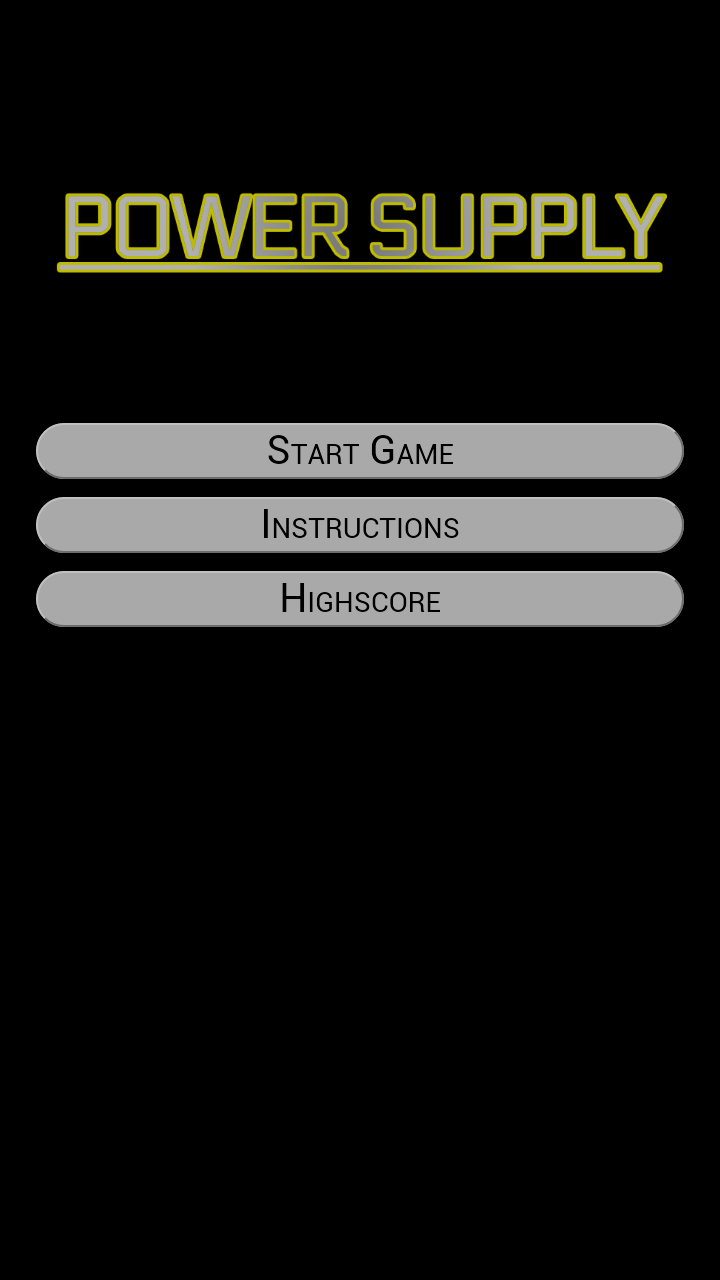
\includegraphics[scale=0.18]{pictures/sprint4-screen/mainmenu}
	}
	\caption{Splash screen when game starts and the game's main menu}
\end{figure}

\begin{figure}[H]
	\centering
	\subfigure{
		
\includegraphics[scale=0.18]{pictures/sprint4-screen/highscore}
	}
	\subfigure{
		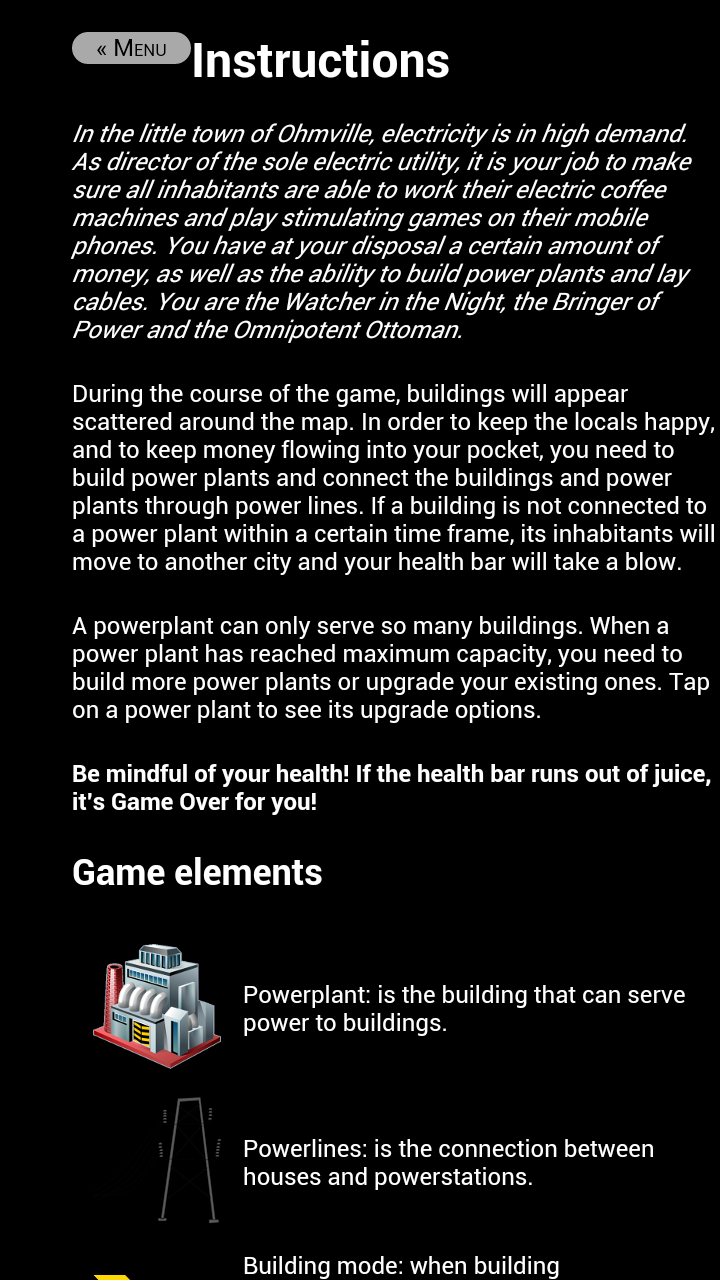
\includegraphics[scale=0.18]{pictures/sprint4-screen/instructions}
	}
	\caption{Highscore and instruction screens}
\end{figure}

\begin{figure}[H]
	\centering
	\subfigure{
		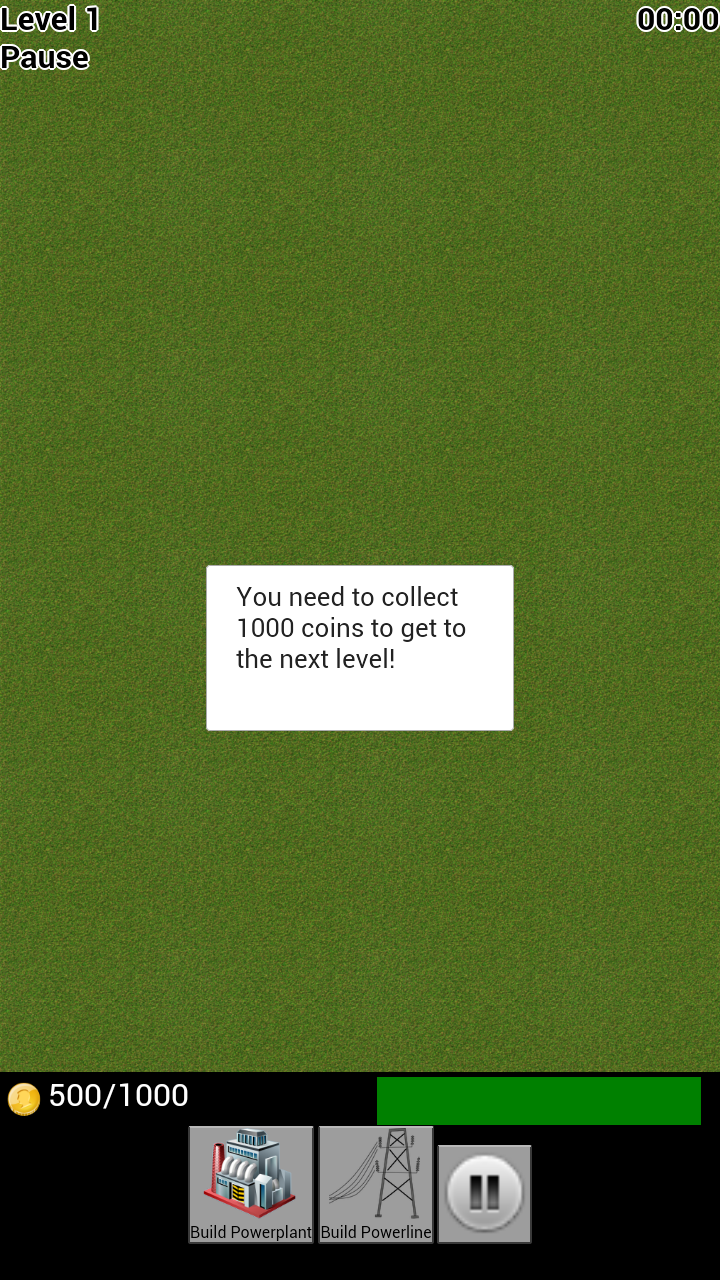
\includegraphics[scale=0.18]{pictures/sprint4-screen/game_start}
	}
	\subfigure{
		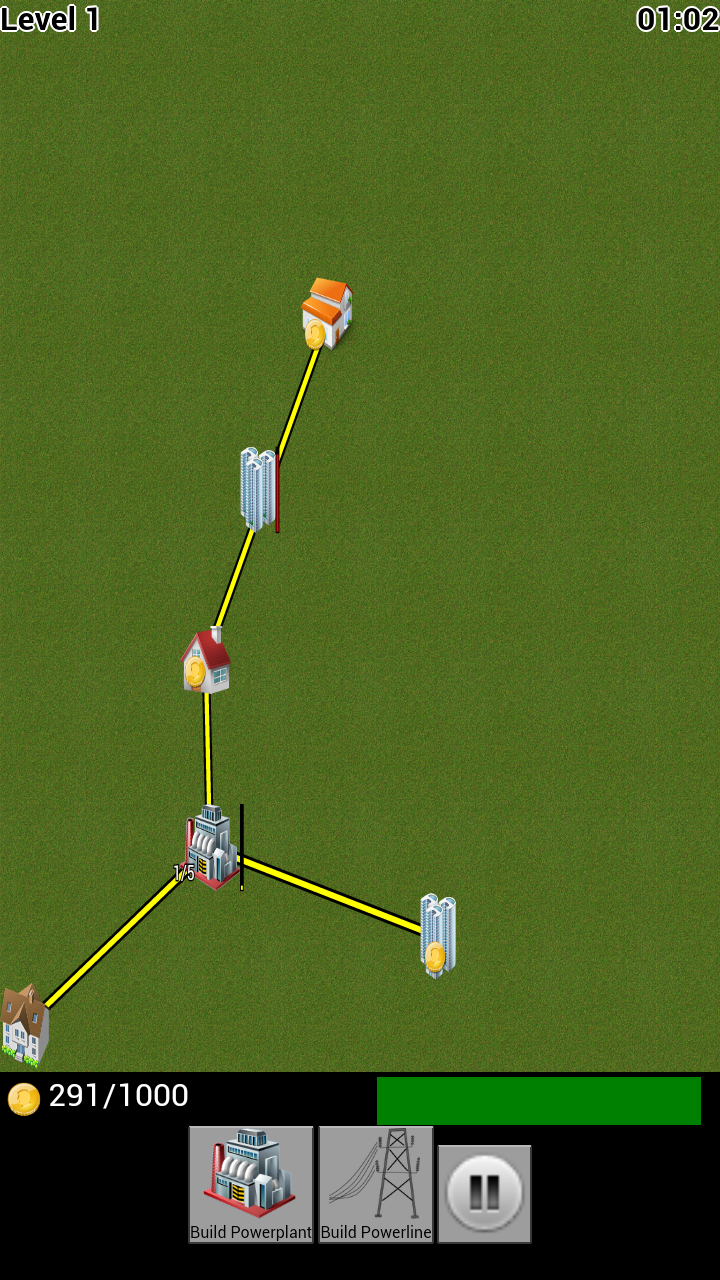
\includegraphics[scale=0.18]{pictures/sprint4-screen/mapoverview}
	}
	\caption{Message when starting a new level and an overview over the map during gameplay}
\end{figure}

\begin{figure}[H]
	\centering
	\subfigure{
		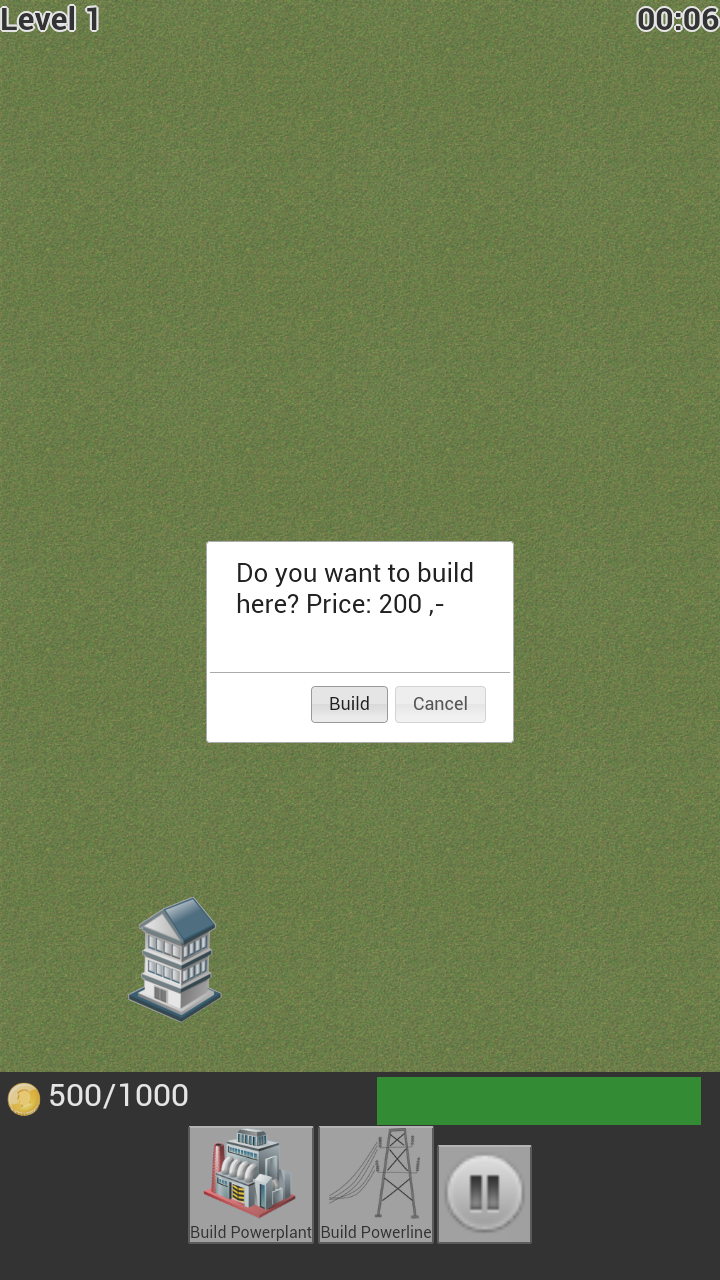
\includegraphics[scale=0.18]{pictures/sprint4-screen/buildpowerplant}
	}
	\subfigure{
		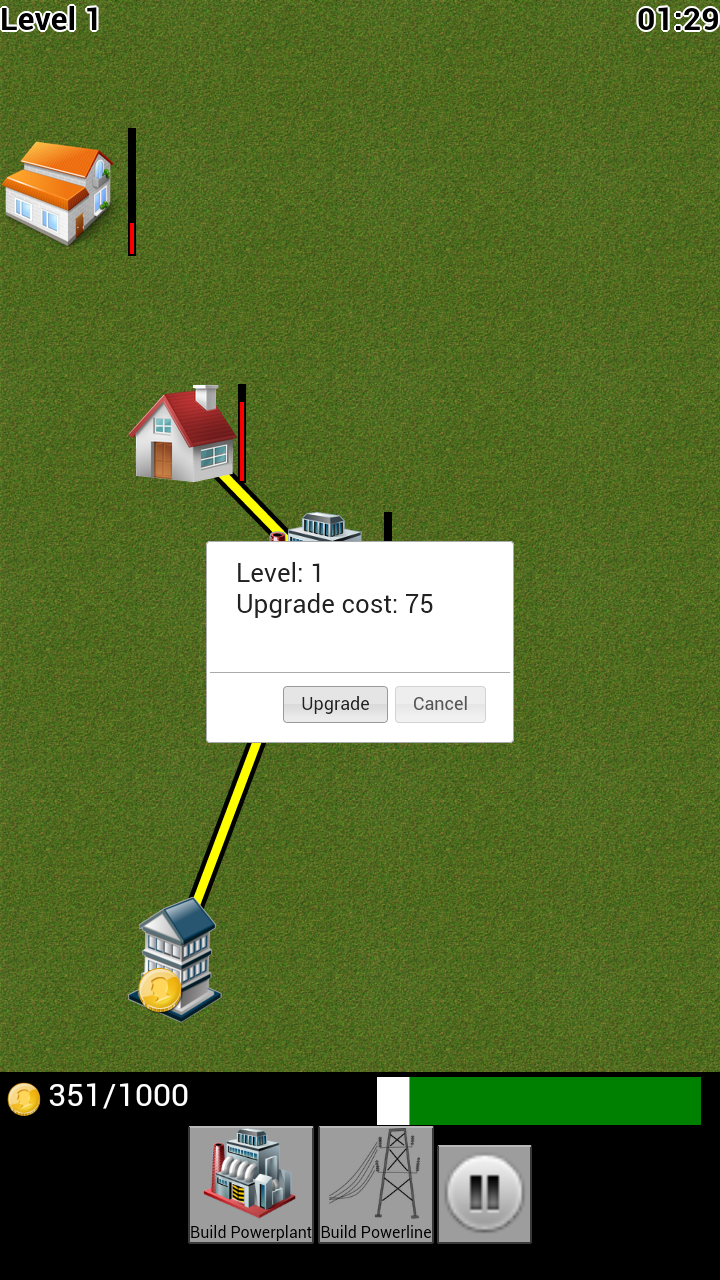
\includegraphics[scale=0.18]{pictures/sprint4-screen/upgradepowerplant}
	}
	\caption{Build and upgrade powerplants}
\end{figure}

\begin{figure}[H]
	\centering
	\subfigure{
		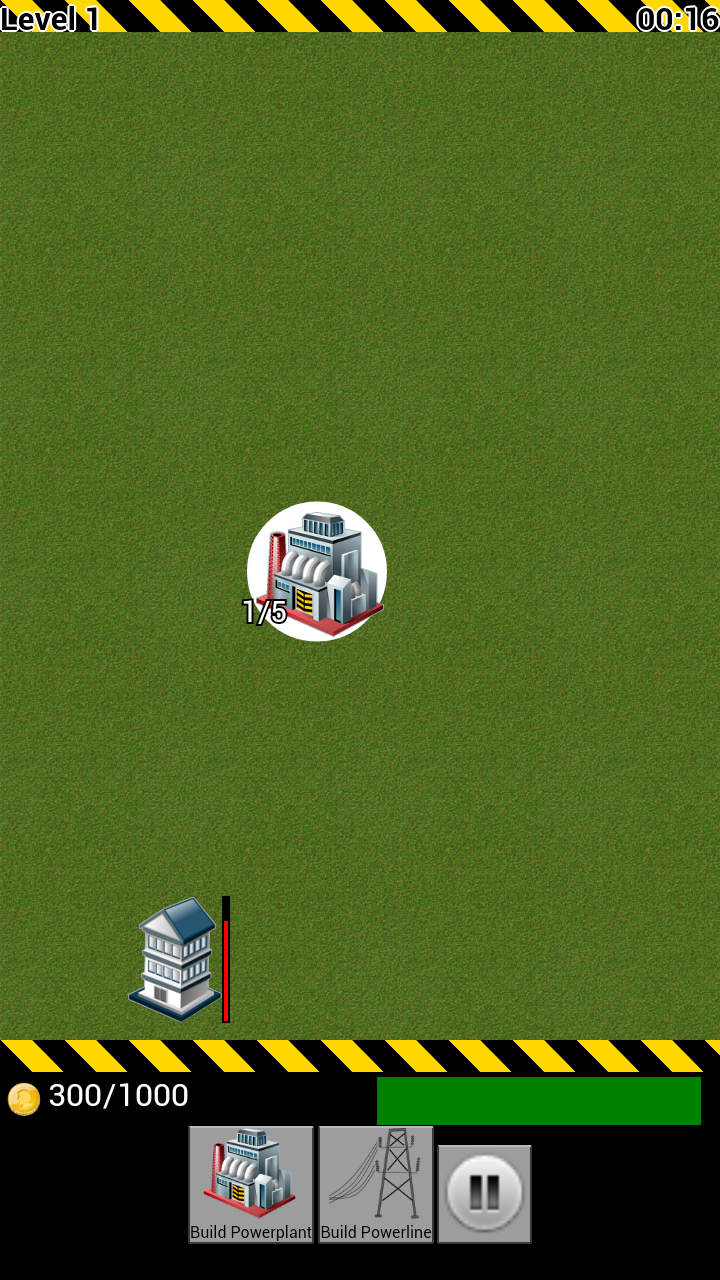
\includegraphics[scale=0.18]{pictures/sprint4-screen/buildpowercable}
	}
	\subfigure{
		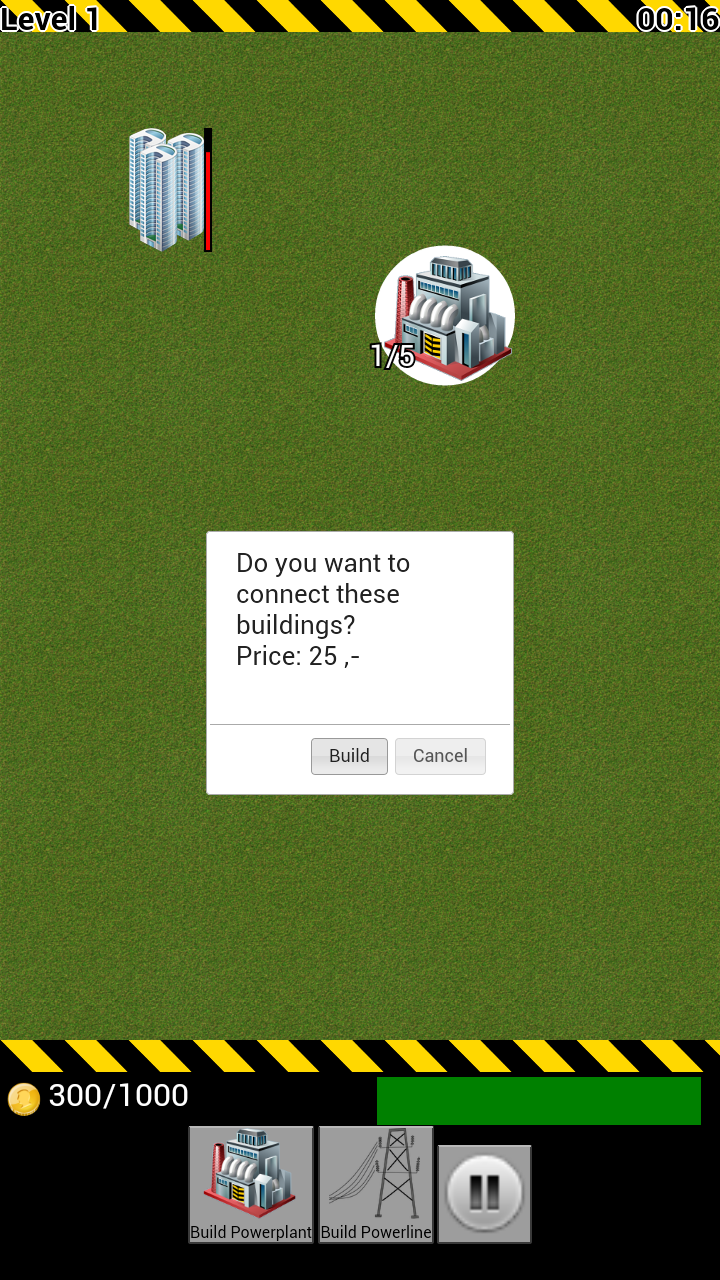
\includegraphics[scale=0.18]{pictures/sprint4-screen/buildpowercable2}
	}
	\caption{Building a power line}
\end{figure}

\begin{figure}[H]
	\centering
	\subfigure{
		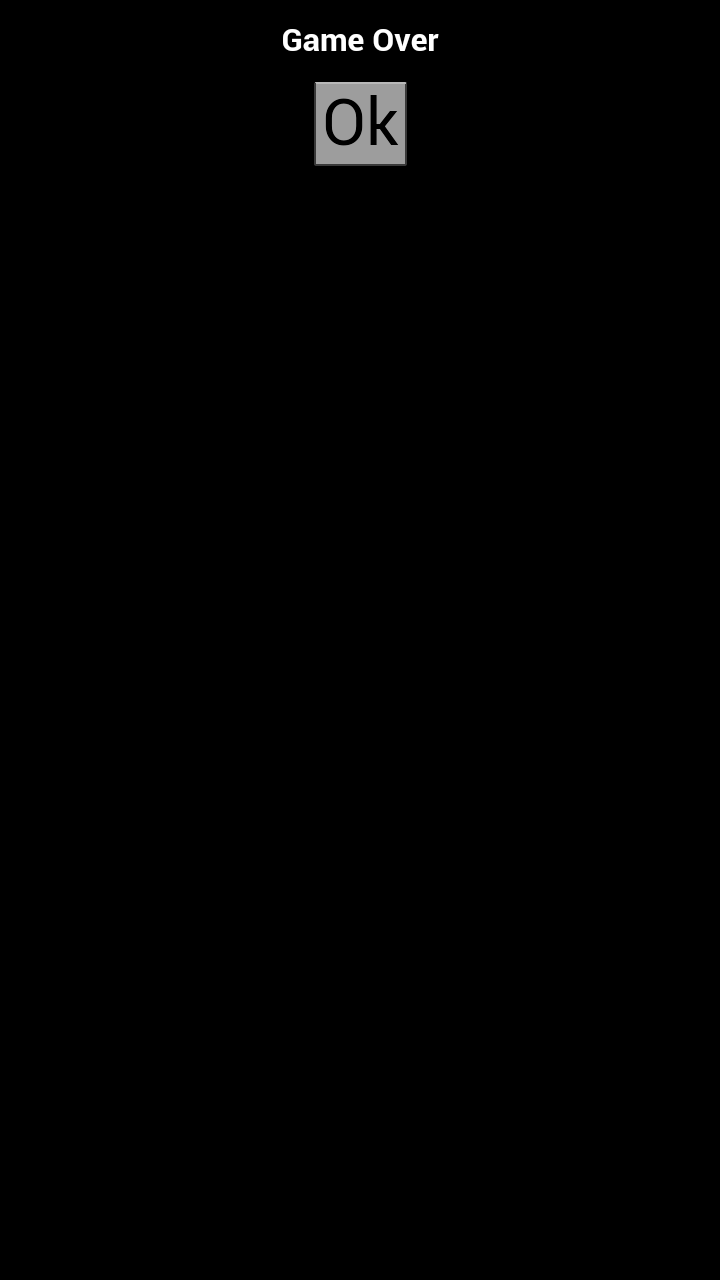
\includegraphics[scale=0.18]{pictures/sprint4-screen/gameover}
	}
	\subfigure{
		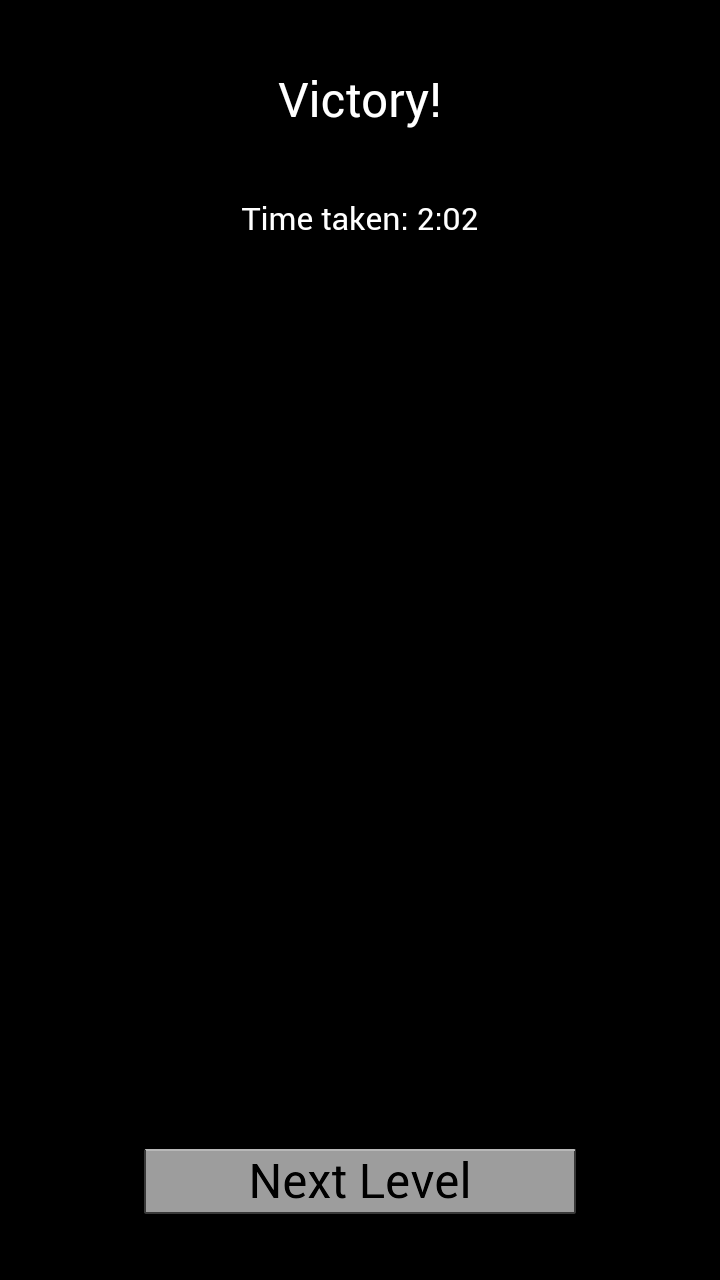
\includegraphics[scale=0.18]{pictures/sprint4-screen/victory}
	}
	\caption{Gameover and victory screens}
\end{figure}


\subsection{Redesign and Bug Fixing}
	
	\subsubsection*{Changes to hud}

		After receiving feedback from the customer and through observations during the usability test in sprint 3, it was decided that the hud was going to be static, i.e. it was not going to be necessary to move it up in order to build. The two icons for building power plants and power lines were made slightly smaller to not make the screen look cluttered.

	\subsubsection*{Scaling GUI elements on iOS}
		Because of differences in screen resolution and in how different browsers
		render HTML content, some pieces of text and images were too large on iOS
		when compared to how they appeared on Android. These issues are not
		technically challenging, generally speaking, but they are quite
		unpredictable and solving them requires some experimentation. All of the
		known layout problems on iOS were solved during this sprint.

	\subsubsection*{Input handling on iOS}
		Because the iOS and Android browsers handle JavaScript TouchEvents
		differently, we had some problems in making map panning work on both
		platforms. This was a fairly subtle bug which took a lot of time to
		understand, but it was solved in the end.

		It turns out that the screen coordinates of a touch event are stored in
		a list of historical touch events, as suggested by the W3C
		documentation\cite{touchEventDocumentation}, in the Android browser.
		On iOS, however, the correct coordinates are only available directly from
		each individual touch object. In order to make panning work well on both
		platforms, we've chosen to detect which platform the app is running on
		and change its behaviour accordingly.

	\subsubsection*{Changed Game logo}
		We did not know which font was used in the first logo, so we changed it to a new
		and better looking one. 

		\begin{figure}
			\centering
			
\includegraphics[scale=0.4]{pictures/logo2.png}
			\caption{Old logo}
		\end{figure}

		\begin{figure}
			\centering
			
\includegraphics[scale=0.4]{pictures/newLogo.png}
			\caption{New logo}
		\end{figure}


\subsection{Testing}

	The test cases listed in Table \ref{table:testssprint4} were executed at the end of this sprint.

	\definecolor{lightgray}{gray}{0.9}

	\begin{table}[H]
	\begin{tabular}{| p{3cm} | p{7cm} | p{2cm} |}
		\hline
		\rowcolor{lightgray}
		{\bf Test Case} & {\bf Result} & {\bf Evaluation} \\ \hline

		FT-25 High score & Works as expected. & Pass. \\ \hline

		FT-26 Pause Game & If one leaves the game while paused the alert follows to the main menu. In order 
		to get anything done in the main menu one need to press 'Resume', which makes the game continue while 
		the player is in the main menu. It can be intuitive for the player to pause the game before going to 
		the main menu, but in the case of our game this works better by just leaving the game. Otherwise the 
		pause function works. & Partially pass. \\ \hline

		FT-27 Sound Effects & It is not possible to mute the music and sounds just for the game. This has to 
		be done by turning off the sound on the phone. Also when exiting the game the background music should 
		stop and then start again when entering the game again. This works for the first time, but not the 
		second time and therefore the background music has been removed. The sounds for damaged power lines and appearing of buildings have not been implemented. The other sounds have been implemented and works as expected. & Partially pass. \\ \hline

		FT-28 Exit Game & If the game is left when a level is completed, but before the next level has been 
		entered, the game returns to main menu and the player needs to start at level 1 again. When exiting 
		the game while in playing mode, it works. & Partially pass. \\ \hline

	\end{tabular}
	\caption{Functional tests from sprint 4}
	\label{table:testssprint4}
	\end{table}

	The test cases in Table \ref{table:retestssprint4} did not pass previous tests and were retested this sprint.

	\begin{table}[H]
	\begin{tabular}{| p{3cm} | p{7cm} | p{2cm} |}
		\hline
		\rowcolor{lightgray}
		{\bf Test Case} & {\bf Result} & {\bf Evaluation} \\ \hline
		
		FT-02 Appearance of buildings & Buildings do not appear on top of each other anymore. & Pass. \\ \hline
		
		FT-05 Build Power Plants & Power Plant are not possible to place on top of other buildings. & Pass. \\ \hline
		
		FT-06 Build Power Lines & There is still no constraints on where power lines can be built as long as it is between two buildings. Otherwise they work. & Partially pass. \\ \hline
		
		FT-20 Damaged Power Lines & Power lines are now possible to fix. & Pass. \\ \hline
	\end{tabular}	
	\caption{Redone tests in sprint 4}
	\label{table:retestssprint4}
	\end{table}

	The test cases that are marked with 'partially pass', works mostly as expected, but has some bugs, errors or missing features that we will not be able to fix before delivery.

	Other bugs that were discovered during testing was that if a building or a power plant is placed 
	too far on the right side on the game map, their bar is not visible to the player. Also after having 
	changed the styling of the dialog box for building power lines, it was no longer possible to decline 
	building a power line when asked, this will be fixed before delivery.

\subsection{Changes to the Requirements}

	Table \ref{table:reqspec4} shows the changes to version 4 of the requirement specification.

	The fact that buildings should not appear on top of each other has finally been added as a requirement, and an additional sound effect requirement has been added.

	Requirement FR1.3 has been removed. The initial plan was that the player could play any level as long as he or she had completed the previous one, and chose which level to play from a menu of all levels. This would be demanding to implement and in addition the levels do not change character to a great extent, only the parameters are changed, from level to level. Therefore it was decided that we will operate with 'tetris-levels', i.e. the player always starts at level 1 and can enter higher levels by winning all previous levels without loosing. 

	\begin{table}[H]
	\begin{tabular}{| p{1.5cm} | p{12cm} |}
		\hline
		\rowcolor{lightgray}
		{\bf FR} & {\bf Change} \\ \hline
		FR1.3 & {\bf \color{red}[REMOVED]}The user should be able to restart any level at any given point of time after start playing. \\ \hline
		FR1.14 & {\bf \color{green}[NEW]} There should be played a sound effect when the player builds a power plant. \\ \hline
		FR2.9 & {\bf \color{green}[NEW]} The houses should not appear on top of each other. \\ \hline
		FR6.14 & {\bf \color{green}[NEW]} The user should be able to click a button, and go into "powerline view mode", where the buildings are not rendered and cannot be interacted with. This is to make it easier to see power lines behind buildings etc. \\ \hline
	\end{tabular}
	\caption{Changes to version 4 of the requirement specification}
	\label{table:reqspec4}
	\end{table}

\subsection{Customer Feedback}

	The customer had tried out the newest version of the product before the
	meeting and was very pleased with it. The customer also said that they did
	not have as easy access to Androids as they had to iPhones, so they had some
	troubles testing the product because we had only given them a download link
	to an Android version and they did not always have an Android at hand.
	However to run it on iPhone they would have to register their phones as
	developer phones with Apple and compile and install the product themselves,
	and we agreed on that it would be even more troublesome. It would have been
	better if the customer had been able to visit us, but because they lived so
	far away we did not feel comfortable calling them down here just to hold a
	15 minute long demo. The customer told us that they had been very pleased
	with how we had controlled the project and that we had always held them well
	informed about the progress of the project and given them frequent
	opportunities to give us feedback.
